\documentclass[12pt, a4paper]{article}

\usepackage{graphicx}
\usepackage{amsmath, amssymb}
\usepackage[utf8]{inputenc}
\usepackage[T2A]{fontenc}
\usepackage[english, russian]{babel}
\usepackage[margin=2cm]{geometry}
\usepackage[most]{tcolorbox}
\usepackage{caption}
\usepackage{enumitem}

\usepackage{cmap}  
\usepackage{textcomp}          % Дополнительные символы

\tcbuselibrary{breakable}
\tcbset{
  width=0.9\textwidth,
  halign=justify,
  center,
  breakable,
  colback=white
}

\title{Билеты к коллоквиуму по математическому анализу}
\author{VG6}
\date{11 неделя 2025}

\newcommand{\N}{\mathbb{N}}
\newcommand{\Q}{\mathbb{Q}}
\newcommand{\Z}{\mathbb{Z}}
\newcommand{\R}{\mathbb{R}}
\newcommand{\eps}{\varepsilon}

\graphicspath{ {./images/} }

\begin{document}
\maketitle
\tableofcontents
\newpage

\section{Введение}
\subsection{Комплексные числа. Действия над ними. Геометрическое представлние. Алгебраическая и триганометрическая форма записи комплексных чисел. Формула Эйлера, определение $e^z$ через действительную экспоненту и действительные триганометрические функции.}

\subsubsection{Определение и свойства}
\begin{tcolorbox}
\textbf{Определение.} \textit{Комплексными числами} называются числа вида $z = x + iy$, где $x, y \in \R$, а $i$ — \textit{мнимая единица}, обладающая свойством $i^2 = -1$.
\end{tcolorbox}
\begin{itemize}
    \item $x = \operatorname{Re } z$ — \textbf{действительная часть} числа $z$.
    \item $y = \operatorname{Im } z$ — \textbf{мнимая часть} числа $z$.
    \item Если $y = 0$, то $z = x$ — действительное число.
    \item Число $\overline{z} = x - iy$ называется \textbf{комплексно-сопряжённым} к $z$.
\end{itemize}

\begin{tcolorbox}
\textbf{Свойство:} $z \cdot \overline{z} = (x + iy)(x - iy) = x^2 - (iy)^2 = x^2 - i^2y^2 = x^2 + y^2$.
\end{tcolorbox}

\begin{tcolorbox}[title=Важное примечание]
\textbf{Нельзя} сравнивать комплексные числа операциями $<, >, \leq, \geq$!
\end{tcolorbox}

\subsubsection{Арифметические операции}
Пусть $z_1 = x_1 + iy_1$, $z_2 = x_2 + iy_2$.
\begin{enumerate}
    \item \textbf{Сложение/Вычитание:}
    $z_1 \pm z_2 = (x_1 \pm x_2) + i(y_1 \pm y_2)$
    \item \textbf{Умножение:}
    \begin{align*}
    z_1 \cdot z_2 &= (x_1 + iy_1)(x_2 + iy_2) = (x_1x_2 - y_1y_2) + i(x_1y_2 + x_2y_1)
    \end{align*}
    \item \textbf{Деление:}
    \begin{align*}
    \frac{z_1}{z_2} &= \frac{(x_1 + iy_1)(x_2 - iy_2)}{(x_2 + iy_2)(x_2 - iy_2)} = \frac{(x_1x_2 + y_1y_2) + i(x_2y_1 - x_1y_2)}{x_2^2 + y_2^2}\\
    \end{align*}
\end{enumerate}

\subsubsection{Геометрическое представление}
\begin{centering}
    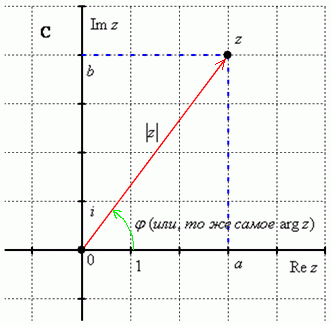
\includegraphics[width=0.4\linewidth]{complex_numbers/compl_plane.png}
\end{figure}

\subsubsection{Тригонометрическая форма}
\begin{tcolorbox}[nobreak]
	\[ z = r(cos\phi +i\; sin\phi),\; r=|z| \]
\end{tcolorbox}

\[ z_1\cdot z_2 = r_1\cdot r_2 \cdot (cos(\phi_1+\phi_2) + i\; sin(\phi_1+\phi_2)) \]
\[\cfrac{z_1}{z_2} = \cfrac{r_1}{r_2}(cos(\phi_1-\phi_2) + i\; sin(\phi_1-\phi_2)) \]

\subsubsection{Формула Эйлера}
\begin{tcolorbox}
	\[ e^{i\phi} = cos\phi +isin\phi \]
	\[ e^z = e^{x+iy} = e^x\cdot e^{iy} = e^x \cdot (cos\; y +i\cdot sin\; y) \]
\end{tcolorbox}

Действительная часть: $ Re\ e^z = e^x \cos y$\\
Мнимая часть: $Im\ e^z = e^x \sin y$


\subsection{Возведение в степень и извлечение корня из комплексных чисел. Форула Муавра.}

\subsubsection{Формула Де-Муавра}
\begin{tcolorbox}
\[ (cos \phi +i\; sin\phi)^k = cos\; k\phi + i\; sin\; k\phi \]
\end{tcolorbox}

\subsubsection{Комплексные корни}
\[ \sqrt[n]{z} = \omega \]
\[ \omega^n = z, z \not= 0\]
\[ z = re^{i\phi}, \omega = \rho e^{i\Psi}  \]
\[ \omega^n = \rho^n e^{in\Psi} = z = re^{i\phi} = re^{i(\phi+2\pi k)}\]
\begin{tcolorbox}
\[ \rho^n = r \Rightarrow \rho = \sqrt[n]{r} \]
\[ n\Psi = \phi + 2\pi k \Rightarrow \Psi = \cfrac{\phi}{n} + \cfrac{2\pi}{n}k \]
\end{tcolorbox}
Корни будут образовывать правильный многоугольник.\\
\begin{centering}
	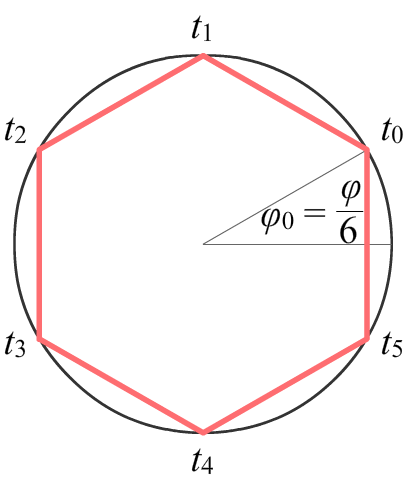
\includegraphics[width=0.2\linewidth]{complex_numbers/roots_of_complex_numbers.png}
\end{centering}

\subsection{Неравенство треугольника для действительных и комплексных чисел, геометрическое и алгебраическое доказательства.}

\subsubsection{Неравенство треугольника}
\begin{figure}[h]
    \centering
    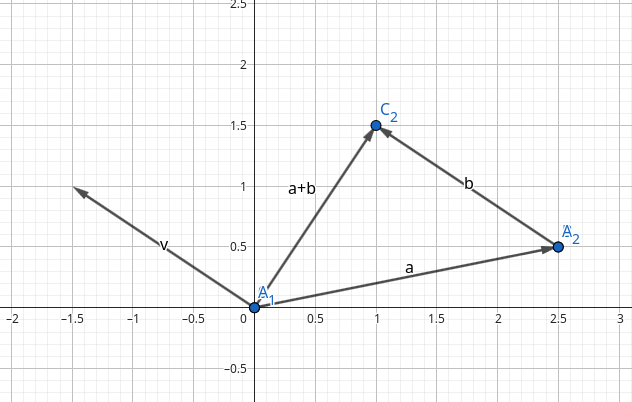
\includegraphics[width=0.5\linewidth]{images/Неравенство(вектора).png}
    \caption{Геометрический смысл неравенства треугольника: длина стороны \( |\vec{a} + \vec{b}| \) не превосходит суммы длин сторон \( |\vec{a}| + |\vec{b}| \).}
    \label{fig:triangle}
\end{figure}
\begin{tcolorbox}
\textbf{Теорема (Неравенство треугольника):}
Для любых комплексных чисел $z_1, z_2$ справедливо:
$$|z_1 + z_2| \leq |z_1| + |z_2|$$
\end{tcolorbox}

\begin{tcolorbox}[title=Доказательство, breakable]
$|a+b| \leq |a| + |b|$
\begin{enumerate}
    \item $a \geq 0\ (|a| \geq |b|)$ \\
    $a + b \geq 0$, то $|a+b| = a+b$.\\
    $a + b \leq 0$, то $|a+b| = -(a+b) = -a-b \leq |a|+|b|$
    \item $|a-b| \geq ||a|-|b||$\\
    $a = (a - b) + b$ по н.т.: $|a + 0| \leq |a-b|+|b| \Rightarrow |a-b| \geq |a|-|b|$ \\
    Аналогично $|b| \leq |b-a|+|a| \Rightarrow |a-b| \geq |b|-|a|$ \\
    Получим, что 
    $
    \begin{cases}
        |a-b| \geq |a|-|b|\\
        |a-b| \geq |-(|a|-|b|)
    \end{cases}
    \Rightarrow |a-b| \geq ||a|-|b||
    $
\end{enumerate}
\end{tcolorbox}

\begin{tcolorbox}[title=Следствие, breakable]
$$||z_1| - |z_2|| \leq |z_1 \pm z_2| \leq |z_1| + |z_2|$$
\end{tcolorbox}

\subsection{Метод математической индукции (ММИ). Прямая индукция. Формула Бинома Ньютона}

\subsubsection{Метод математической индукции (ММИ)}
\begin{tcolorbox}
\textbf{Алгоритм доказательства по индукции:}
\begin{enumerate}
    \item \textbf{База индукции:} Проверить утверждение для $n = 1$.
    \item \textbf{Индукционное предположение:} Предположить, что утверждение верно для $n = k$.
    \item \textbf{Индукционный переход:} Доказать, что из этого следует верность утверждения для $n = k+1$ (Прямая индукция).
\end{enumerate}
\end{tcolorbox}

\subsubsection{Бином Ньютона}
\begin{tcolorbox}
\textbf{Определение.}\\
\textit{Биномиальный коэффициент}:
$C_n^k = \dfrac{n!}{k!(n-k)!}$, где $n,k \in \mathbb{N}_0$\\
\end{tcolorbox}

\begin{tcolorbox}
\textbf{Формула бинома Ньютона:}
$$(a+b)^n = \sum_{k=0}^{n} C_n^k a^{n-k}b^k$$
\end{tcolorbox}

\begin{tcolorbox}[title=Доказательство по ММИ, breakable]
\textbf{База индукции:} Для $n=1$:
$$(a+b)^1 = a + b$$
$$\sum_{k=0}^{1} C_1^k a^{1-k}b^k = C_1^0 a^1 b^0 + C_1^1 a^0 b^1 = 1 \cdot a \cdot 1 + 1 \cdot 1 \cdot b = a + b$$
База индукции доказана.

\textbf{Индукционное предположение:} Предположим, формула верна для $n = m$:
$$(a+b)^m = \sum_{k=0}^{m} C_m^k a^{m-k}b^k$$

\textbf{Индукционный переход:} Докажем для $n = m+1$.
Рассмотрим левую часть:
$$(a+b)^{m+1} = (a+b) \cdot \sum_{k=0}^{m} C_m^k a^{m-k}b^k$$
Раскроем скобки:
$$= \sum_{k=0}^{m} C_m^k a^{m+1-k}b^k + \sum_{k=0}^{m} C_m^k a^{m-k}b^{k+1}$$
Во второй сумме сделаем замену индекса $j = k+1$:
$$= \sum_{k=0}^{m} C_m^k a^{m+1-k}b^k + \sum_{j=1}^{m+1} C_m^{j-1} a^{m+1-j}b^{j}$$
Теперь объединим суммы, выделяя крайние слагаемые:
$$= C_m^0 a^{m+1} + \sum_{k=1}^{m} \left[ C_m^k + C_m^{k-1} \right] a^{(m+1)-k}b^k + C_m^m b^{m+1}$$
Используем свойство биномиальных коэффициентов:
$$C_m^k + C_m^{k-1} = C_{m+1}^k$$
Учитывая, что $C_m^0 = C_{m+1}^0 = 1$ и $C_m^m = C_{m+1}^{m+1} = 1$, получаем:
$$(a+b)^{m+1} = \sum_{k=0}^{m+1} C_{m+1}^k a^{(m+1)-k}b^k$$
Индукционный переход завершён.
\end{tcolorbox}

\subsection{ММИ. Обратная индукция. Неравенство между средним арифметическим и средним геометрическим.}

\subsubsection*{Неравенство о средних}
\begin{tcolorbox}
\textbf{Теорема (Неравенство между средним арифметическим и средним геометрическим):}
Для любых $a_1, a_2, \dots, a_n \geq 0$ справедливо:
$$\frac{a_1 + a_2 + \dots + a_n}{n} \geq \sqrt[n]{a_1 a_2 \dots a_n}$$
Равенство достигается тогда и только тогда, когда $a_1 = a_2 = \dots = a_n$.
\end{tcolorbox}

\begin{tcolorbox}[title=Доказательство по ММИ (метод Коши / метод обратой индукции), breakable]
Докажем теорему в три этапа.

\textbf{1. База индукции для степеней двойки ($n=2^m$).}
\begin{itemize}
    \item \textbf{Для $n=2$:} Докажем $\frac{a_1 + a_2}{2} \geq \sqrt{a_1 a_2}$.
    $$(a_1 - a_2)^2 \geq 0 \Rightarrow a_1^2 - 2a_1a_2 + a_2^2 \geq 0 \Rightarrow a_1^2 + 2a_1a_2 + a_2^2 \geq 4a_1a_2 \Rightarrow$$
    $$\Rightarrow (a_1 + a_2)^2 \geq 4a_1a_2 \Rightarrow \frac{a_1 + a_2}{2} \geq \sqrt{a_1 a_2}$$
    \item \textbf{Предположим, неравенство верно для $n = k$.}
    \item \textbf{Докажем для $n = 2k$:}
    $$\frac{a_1 + \dots + a_{2k}}{2k} = \frac{\frac{a_1 + \dots + a_k}{k} + \frac{a_{k+1} + \dots + a_{2k}}{k}}{2} \geq$$
    $$\geq \frac{\sqrt[k]{a_1 \dots a_k} + \sqrt[k]{a_{k+1} \dots a_{2k}}}{2} \geq \sqrt{\sqrt[k]{a_1 \dots a_k} \cdot \sqrt[k]{a_{k+1} \dots a_{2k}}} = \sqrt[2k]{a_1 \dots a_{2k}}$$
\end{itemize}

\textbf{2. Докажем, что если неравенство верно для $n$, то оно верно и для $n-1$.}
Рассмотрим $a_1, a_2, \dots, a_{n-1} \geq 0$. Пусть
$$a_n = \frac{a_1 + a_2 + \dots + a_{n-1}}{n-1}$$
Для набора из $n$ чисел неравенство верно:
$$\frac{a_1 + \dots + a_{n-1} + a_n}{n} \geq \sqrt[n]{a_1 a_2 \dots a_{n-1} a_n}$$
Подставим $a_n$:
$$\frac{(a_1 + \dots + a_{n-1}) + \frac{a_1 + \dots + a_{n-1}}{n-1}}{n} = \frac{a_1 + \dots + a_{n-1}}{n-1} = a_n$$
Таким образом:
$$a_n \geq \sqrt[n]{a_1 a_2 \dots a_{n-1} a_n}$$
Возведём в степень $n$:
$$a_n^n \geq a_1 a_2 \dots a_{n-1} a_n \Rightarrow a_n^{n-1} \geq a_1 a_2 \dots a_{n-1}$$
Извлекая корень $(n-1)$-й степени:
$$a_n \geq \sqrt[n-1]{a_1 a_2 \dots a_{n-1}} \Rightarrow \frac{a_1 + \dots + a_{n-1}}{n-1} \geq \sqrt[n-1]{a_1 a_2 \dots a_{n-1}}$$

\textbf{3. Завершение доказательства.}
Мы доказали, что:
\begin{enumerate}
    \item Неравенство верно для $n=2$ (а значит, для $n=4,8,16,\dots$)
    \item Из верности для $n$ следует верность для $n-1$
\end{enumerate}
Следовательно, неравенство верно для любого натурального $n$.
\end{tcolorbox}

\section{Действительные чсла. Числовые множества.}
\subsection{Дедекиндовы сечения. Определение действительных чисел по Дедекинду. Полнота $\R$ по Дедекинду.}
\subsection{Лемма об отделимости.}
\subsection{Точная верхняя и нижняя грани ограниченных множеств из В.
Теорема Вейерштрасса о существовании точной верхней грани
ограниченного сверху множества как следствие леммы об отде-
лимости (принцип полноты В по Вейерштрассу).}
\subsection{Последовательности стягивающихся отрезков с действительны-
ми концами. Теорема Кантора о стягивающихся отрезках с дей-
ствительными концами (принцип полноты ® по Кантору).}
\subsection{Полнота К по Дедекинду как следствие принципа стягивающихся
отрезков.}
\subsection{Счётность множества, рациональных чисел и несчётность множества действительных чисел.}
\section{Последовательность и ряды.}

\subsection{Свойства сходящихся последовательностей (сходимость постоянной последовательности, единственность предела, ограниченность сходящейся последовательности).}
\subsection{Предельный переход в неравенствах для последовательностей.}
\subsection{Теорема о зажатой последовательности (о трёх последовательностях).}
\subsection{Теоремы о сохранении знака сходящейся последовательностью и о сходимости модулей.}
\subsection{Бесконечно малые последовательности, их свойства.}
\subsection{Бесконечно большие последовательности. Связь бесконечно малых и бесконечно больших последовательностей.}
\subsection{Арифметические свойства сходящихся последовательностей.}
\subsection{Монотонные последовательности. Критерий сходимо}сти монотонной последовательности.
\subsection{Число е как предел последовательности.}
\subsection{Теорема Больцано-Вейерштрасса.}
\subsection{Частичные пределы. Критерий частичного предела.}
\subsection{Критерий Коши существования предела последовательности.}
\subsection{Существование верхнего и нижнего пределов у любой последовательности.}
\subsection{Числовые ряды. Абсолютная и условная сходимость числовых рялов. Критерий Коши сходимости ряда. Необходимое условие сходимости ряда. Признак сравнения.}
\subsection{Признаки абсолютной сходимости рядов Даламбера и Коши.}


\subsection{Критерий Коши сходимости ряда с монотонными членами. Исследование сходимости ряда $ \sum_{n = 1}^{\infty} \frac{1}{n^p},\ p > 0 $.}

\end{document}
